\subsection{Wägezelle}

In diesem Versuch wird eine Wägezelle mit dem Wägesensor HX711 eingesetzt, der in \autoref{fig:HX711} dargestellt ist.
Der Sensor HX711 ist ein Analog-Digital-Wandler, der die analogen Spannungsänderungen der Wheatstone-Brücke verstärkt und in ein digitales Signal umwandelt.
Dieses digitale Signal kann dann von einem Mikrocontroller verarbeitet werden.
In diesem Projekt wird der Arduino Nano verwendet wie in \autoref{fig:Nano-Pinlayout} dargestellt.
\\
% \begin{center}
%     \centering
%     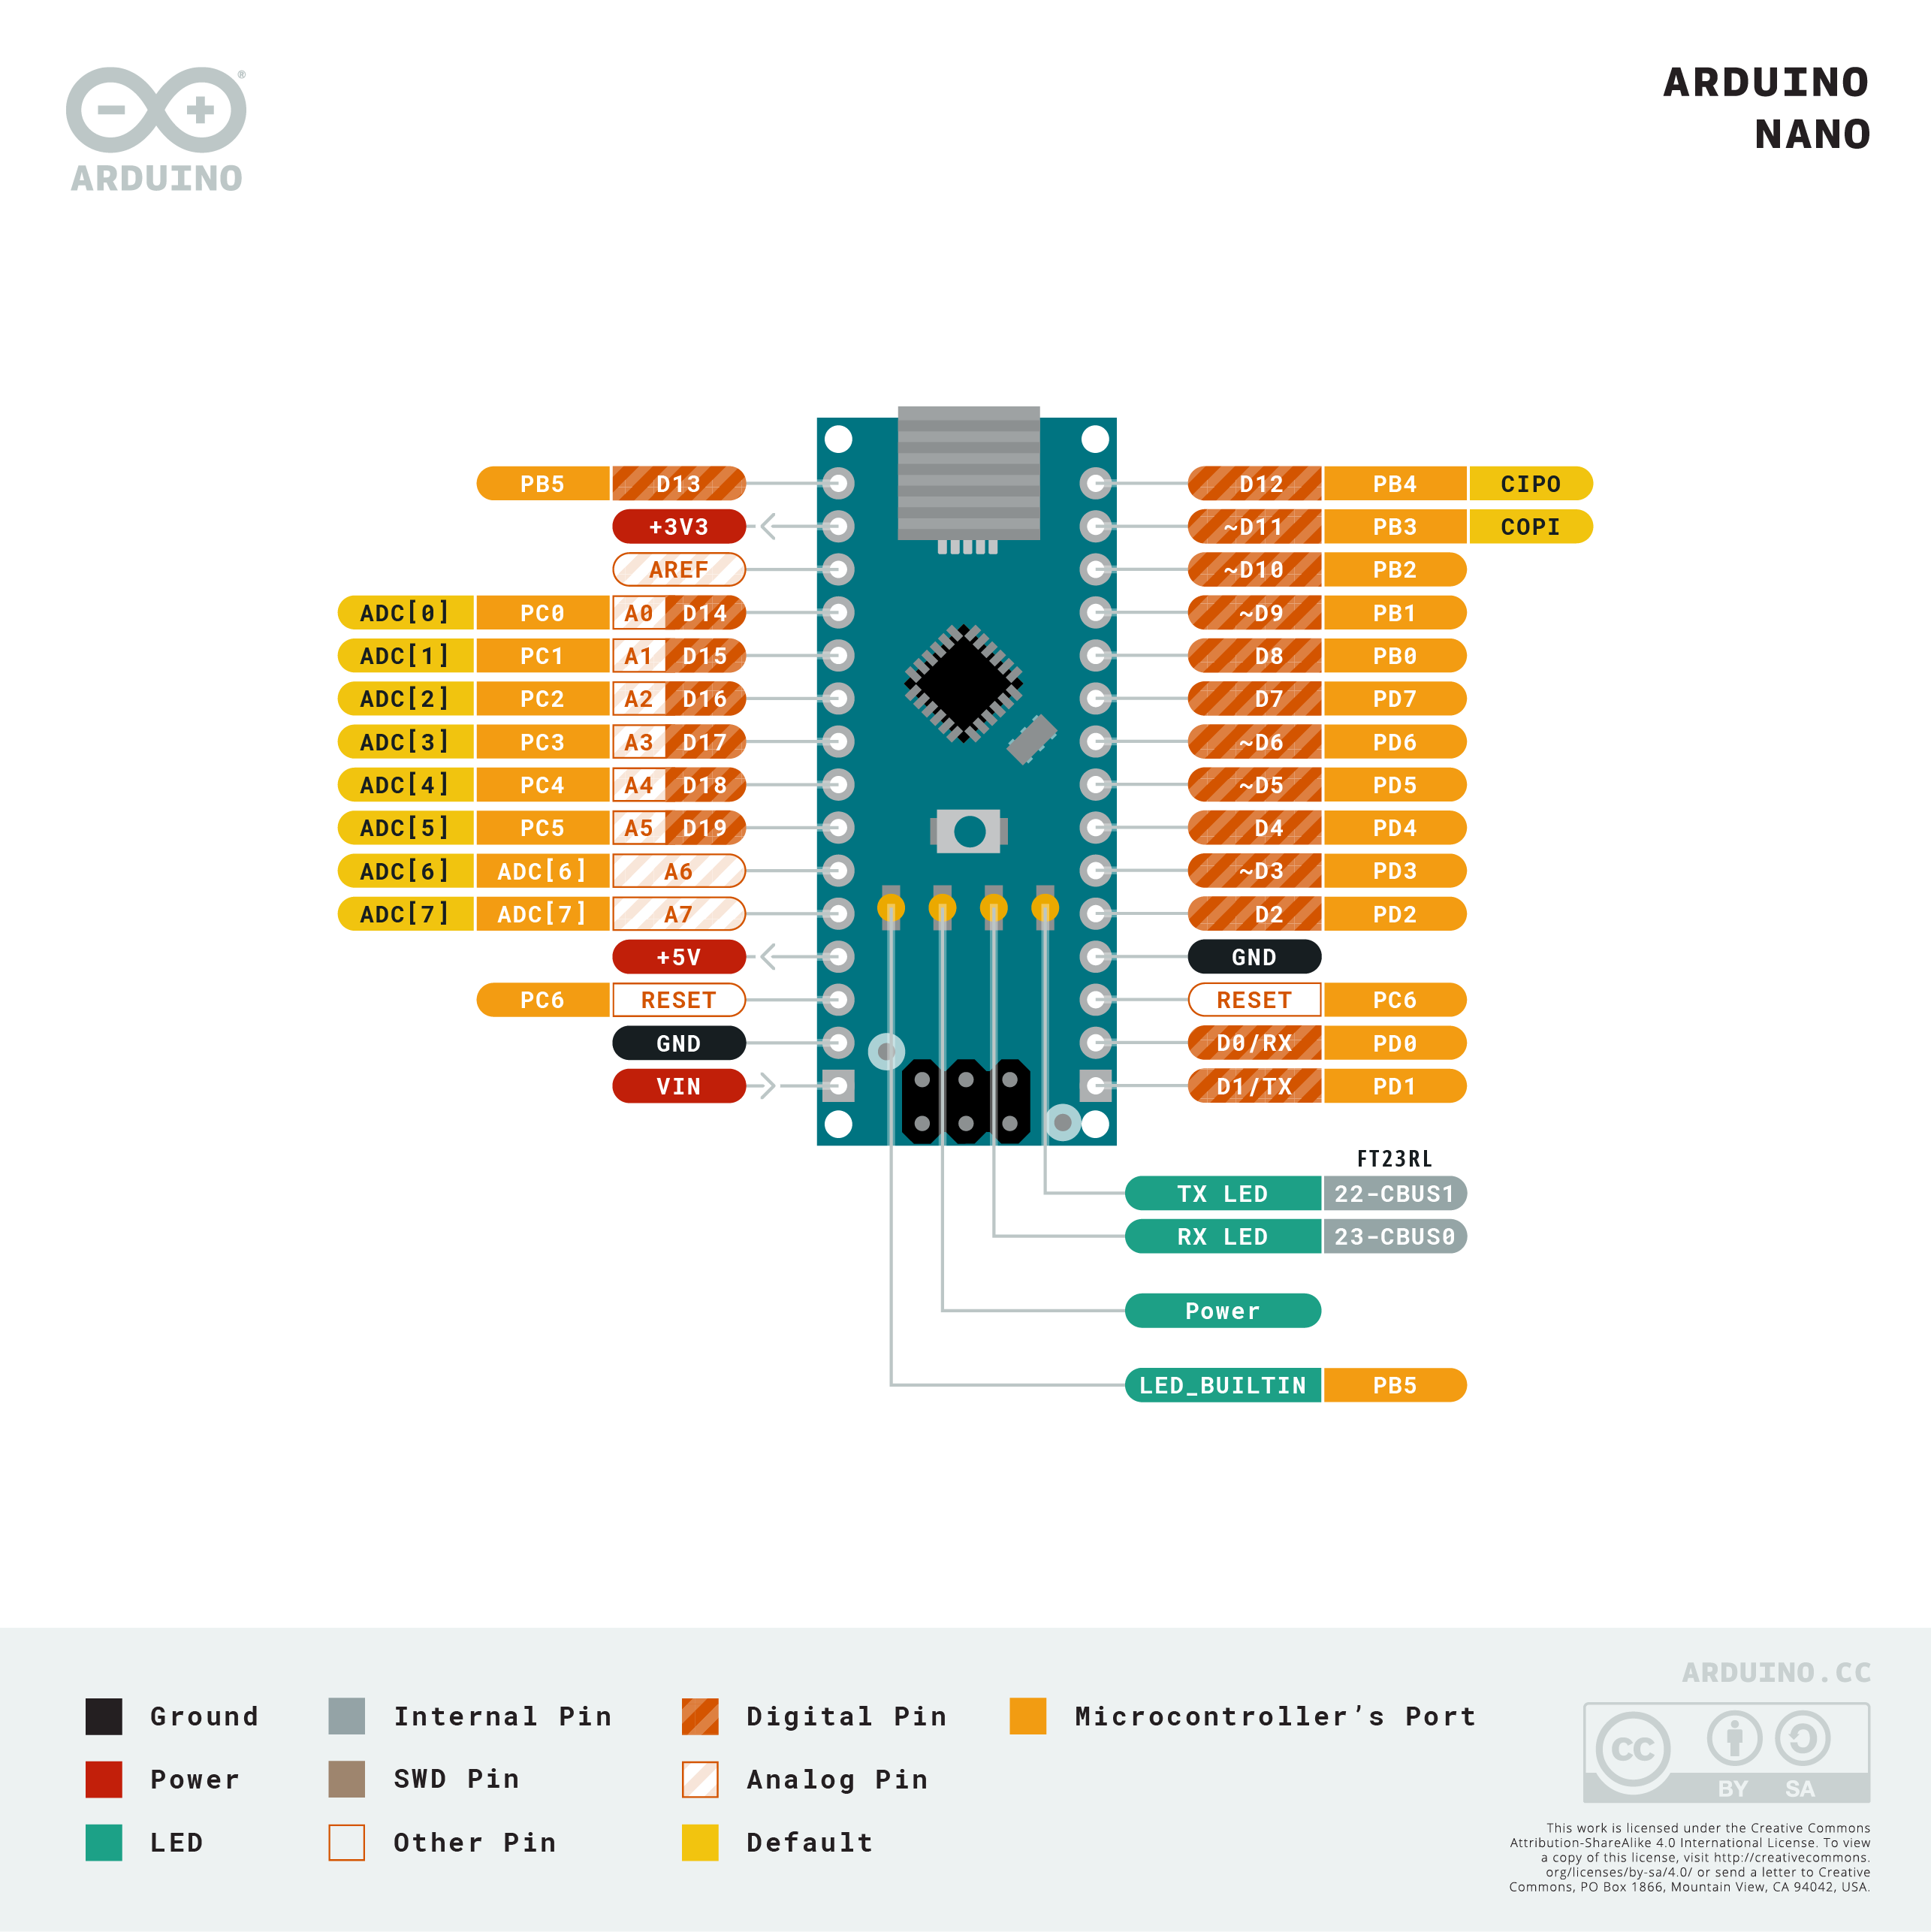
\includegraphics[width=0.9\textwidth]{img/Nano-Pinlayout.png}
%     \captionof{figure}[Nano-Pinlayout ]{Nano-Pinlayout \cite{Arduino}}
%     \label{Nano-Pinlayout}
% \end{center}

% \begin{center}
%     \centering
%     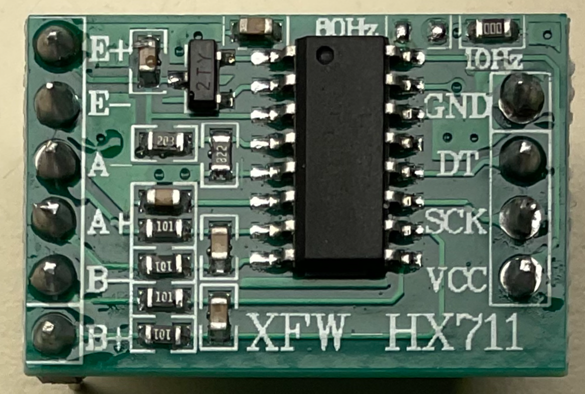
\includegraphics[width=0.6\textwidth]{img/HX711.png}
%     \captionof{figure}[HX711]{HX711 \cite{prilchen}}
%     \label{HX711}
% \end{center}
Um die Signale der Wägezelle an den HX711 weiterzugeben, die Signale des HX711 mit dem Arduino Nano zu verarbeiten und die Daten lesbar darzustellen, müssen die drei Komponenten miteinander verschaltet werden und korrekt kommunizieren.
\\
Zuerst wird die Wägezelle an eine 5 V Gleichstromquelle angeschlossen und dann mit dem HX711 verbunden. Wodurch die Wägezelle die analogen Signale an den HX711 weitergeben kann. Der HX711 wandelt sie dann in ein digitales Signal und gibt dieses an den Arduino Nano weiter. Der VCC-Pin HX711 wird mit dem 5V-Pin des Arduino Nano verbunden. Der GND-Pin mit dem GND-Pin des Ardiunos. Der DT-Pin ist der Datenausgang des HX711 und wird mit irgendeinem der Digital-Pins des Nanos verbunden, genauso wie der SCK-Pin, z.B. $DT-Pin -> D3-Pin$ und $SCK-Pin -> D2-Pin$. Der SCK-Pin oder serial-clock-Pin steuert die Übertragung des Signals des DT-Pins. Der Arduino gibt auf dem SCK-Pin den Takt vor, mit dem der HX711 die Daten an den Mikrocontroller sendet. Der Ardiuno setzt den SCK-Pin auf high und dann wieder auf low. Dieser Wechsel, vom Ende eines low-Signals zu einem high- und wieder einem low-Signal ist ein Takt. Der HX711 sendet dann pro Takt ein Bit, also einen low-Puls für 0 und einen high-Puls für 1.
\\
\\
Der Arduino-Nano wird dann an einen Computer angeschlossen.
In der Arduino IDE können mithilfe der passenden Library und einem Code die Daten ausgelesen und gespeichert werden.
\begin{figure}[h!]
    \centering
    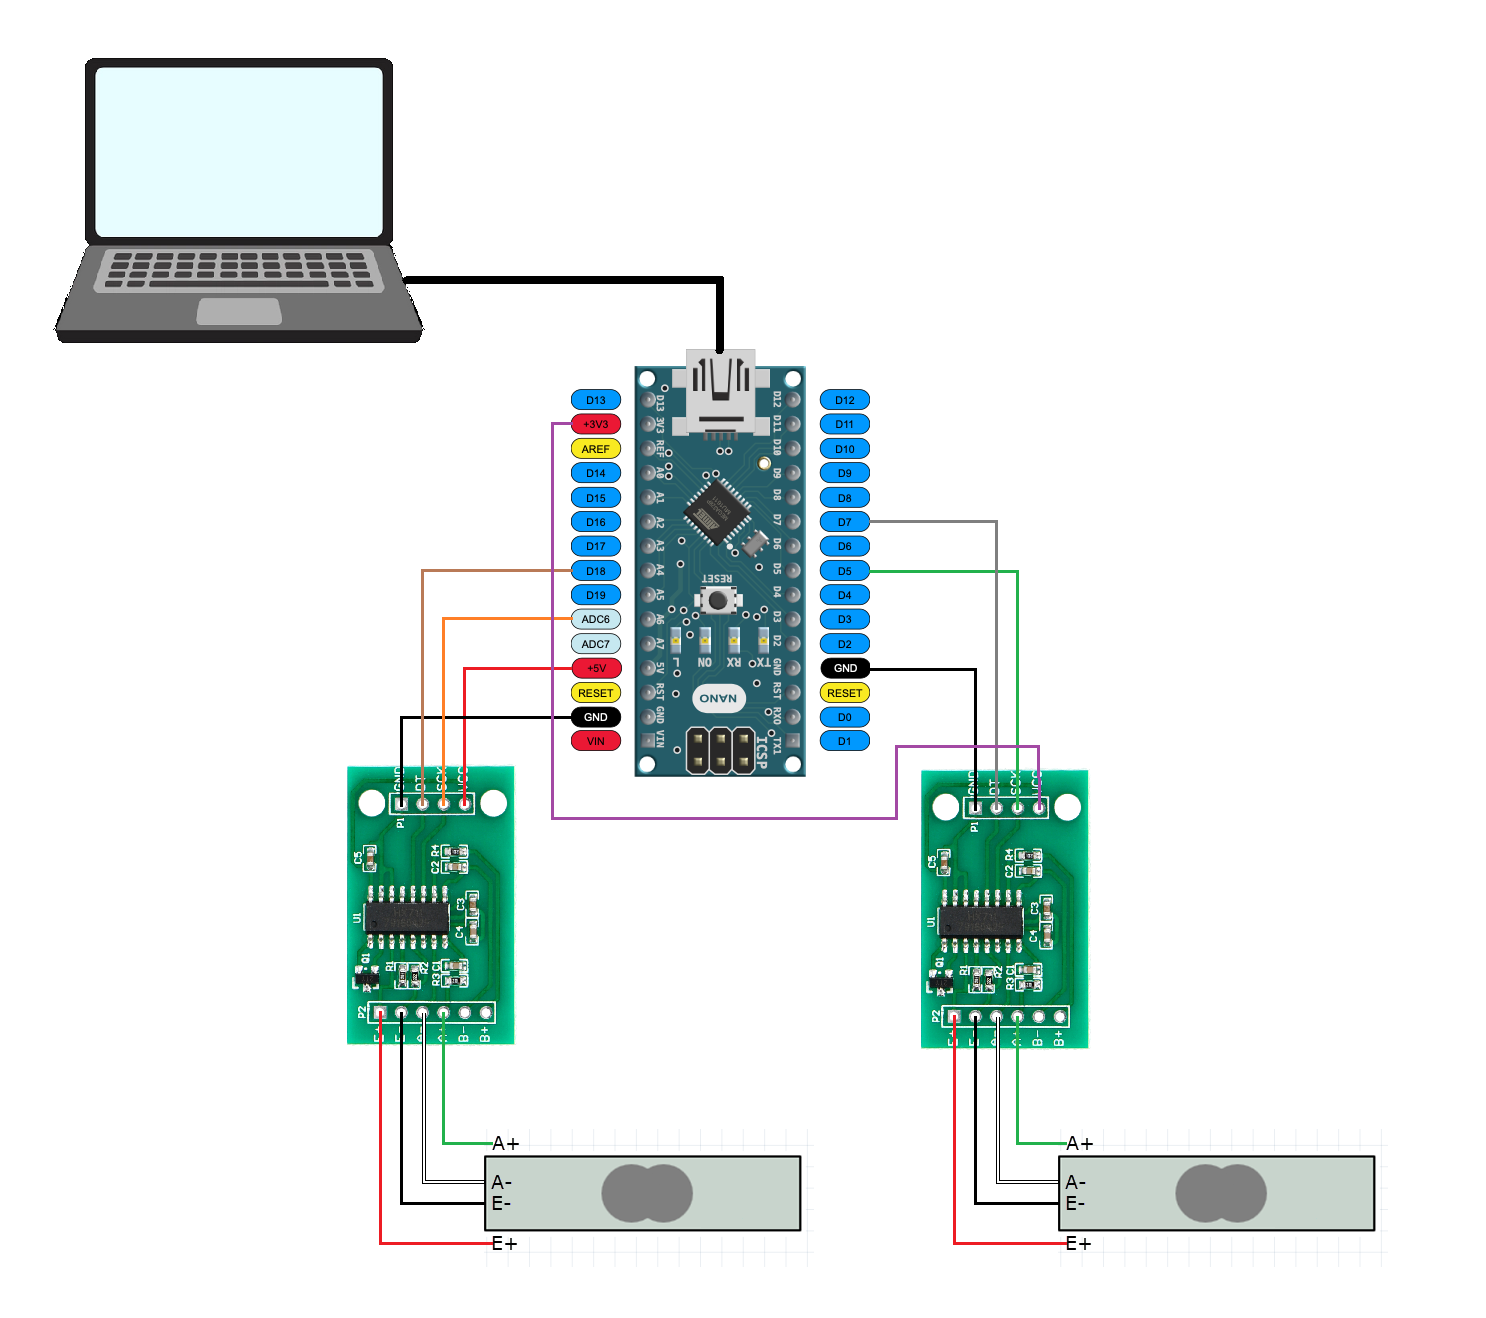
\includegraphics[width=0.8\textwidth]{img/Schaltungs-Aufbau.png}
    \caption{Gesamtaufbau Wägezelle mit Arduino Nano}
    \label{Gesamtaufbau-waegezelle-mit-Arduino-Nano}
\end{figure}
\\
Der auf dem Arduino ausgeführte C-Code liest periodisch den analogen Wert des HX711 aus. Zunächst muss der Sensor initialisiert werden. Dies geschieht durch:
\begin{enumerate}
    \item \textbf{Angabe eines Kalibrationswertes}: Dieser Wert dient der genauen Gewichtsmessung.
    \item \textbf{Tara-Einstellung}: Die Waage wird auf 0 kg gesetzt, um sicherzustellen, dass nachfolgende Messungen korrekt sind.
\end{enumerate}
Nach der Initialisierung ist die Waage bereit, Messdaten auszugeben.
\\
Für die Ausgabe eines Messwerts werden die gemessenen Daten über den Serial-Port übertragen.
Dabei wird angegeben, ob die Messung von der linken oder rechten Waage stammt.
Die Ausgabe erfolgt beispielsweise wie folgt:
\begin{center}
    \texttt{Gewicht rechts [kg]: -0.00118}  \\
    \texttt{Gewicht links [kg]: -0.00321} \\
    \texttt{Gewicht rechts [kg]: -0.00118} \\
    \texttt{Gewicht links [kg]: -0.00223} \\
\end{center}
Der serielle Monitor verarbeitet die Ausgabe des Arduinos und ergänzt jeden Messwert mit einem Zeitstempel, der den Zeitpunkt angibt, zu dem der Messwert den Computer erreicht. Dadurch wird es möglich, die seriellen Daten in Echtzeit als Graph über die Zeit darzustellen, wie in \autoref{fig:serial_output_example} veranschaulicht.
%todo:
\begin{figure}[h!]
    \centering
    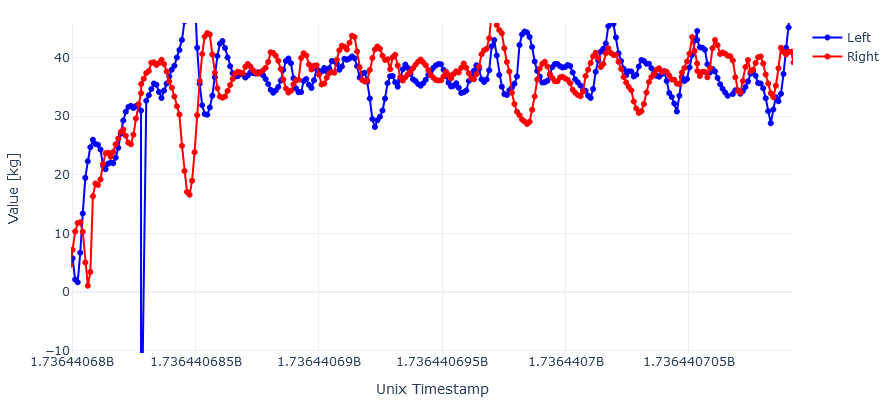
\includegraphics[width=0.7\textwidth]{img/serial_output_example.png} % Screenshot oder Beispiel
    \caption{Ausgabe der Messdaten mit Python}
    \label{fig:serial_output_example}
\end{figure}
\\
Allen Daten werden in einem CSV-Format gespeichert.
Sie können nun beliebig aufbereitet und analysiert werden.
% Der C Code auf dem Arduino liest periodisch den analogen Wert des HX711 aus, muss dafür aber zuerst initialisiert werden.
% Dazu wird ein Kalibrationswert angegeben und anschließend die Waage auf 0 kg getared.
% Nun ist die Waage initialisiert und bereit, Messdaten auszugeben.
% Soll ein Messwert ausgegeben werden, so werden die Daten an den Serial-Port ausgegeben, mit dem Hinweis, ob der Messwert von links oder rechts stammt.
% \begin{center}
%     Gewicht links: ...  \\
%     Gewicht rechts: ...
% \end{center}
% An dem Serial-Port angekommen werden die Daten von einem zweiten parallel laufenden Python Skript ausgewertet.
% Dabei können die Daten in Echtzeit in einer web App dargestellt werden und werden gleichzeitig aufgezeichnet im CSV-Format.
% \\
% Diese Daten können nun auf verschiedene Art und Weisen mithilfe von Python dargestellt werden.


\subsection{EMG Messung}

\begin{figure}[h!]
    \centering
    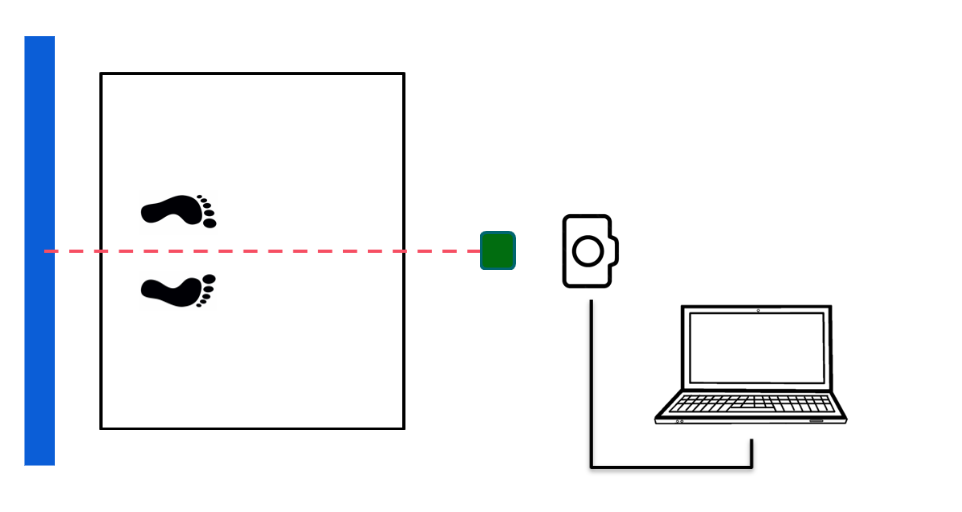
\includegraphics[width=0.8\linewidth]{img/Aufbau-EMG.png}
    \caption{EMG Messaufbau}
    \label{fig:EMG-Messaufbau}
\end{figure}

Im Rahmen des Messversuchsaufbaus, dargestellt in \autoref{fig:EMG-Messaufbau} wurde zunächst sichergestellt, dass die Probanden eine reproduzierbare Ausgangsposition für die Kniebeuge einnehmen konnten.
Hierzu wurden die Fußumrisse jedes Probanden auf einem großen Papier aufgezeichnet.
Dies diente als Orientierungshilfe, um die Standposition exakt wiederherstellen zu können.
\\
\\
Zur korrekten Ausrichtung während der Bewegung wurde ein Baulaser in einer Entfernung von 1,5 Metern vor dem Probanden positioniert. Dieser projizierte eine vertikale Linie, an der sich die Probanden vor jeder Messung neu ausrichten konnten. Hinter dem Baulaser wurde eine Kamera installiert, die synchron mit einem PC und dem EMG-Messsystem (Elektromyografie) verbunden war.
\\
Für eine konsistente Bild- und Datenaufnahme wurde im Hintergrund ein Zeichenboard als gleichfarbige Kulisse positioniert. Dies minimierte störende visuelle Einflüsse und erleichterte die anschließende Auswertung der aufgenommenen Daten.
Die EMG-Elektroden wurden gezielt am Quadrizeps platziert, um die Muskelaktivität differenziert zu messen. Dabei wurden drei spezifische Positionen am Oberschenkel berücksichtigt: innen am Vastus medialis, mittig am Rectus femoris und außen am Vastus lateralis. An jedem Bein wurden jeweils eine Elektrode am rechten und linken Oberschenkel angebracht, um eine beidseitige Erfassung der Muskelaktivität während der Kniebeuge sicherzustellen.

